\chapter{PRBS modelling and implementation of pole-placement controller}
The first half of this chapter is dedicated to do system identification of the SBHS system using the response obtained for a PRBS (Pseudo Random Binary Sequence) input. In the second half, a pole-placement controller is designed using this model and implemented on SBHS.


\section{PRBS testing}

Similar to Chapter \ref{chap1} and \ref{chap2}, in this section we will find the transfer function model of SBHS. But there are two major differences. First difference is that we will give a Pseudo Random Binary Sequence to the heater input of SBHS and second difference is that we will find the discrete time transfer function. A Pseudo Random Binary Sequence is nothing but a signal whose amplitude varies between two limits randomly at any given time. An illustration of the same is given in figure \ref{prbs-fig}. A PRBS signal can be easily generated using the $rand()$ function in scilab. Scilab code to generate the PRBS signal is given at the end of this chapter. Figure \ref{prbs-xcos} shows the xcos diagram for PRBS testing. The PRBS amplitude and offset value to the input can be adjusted using the rlevant blocks.
\begin{figure}
\centering
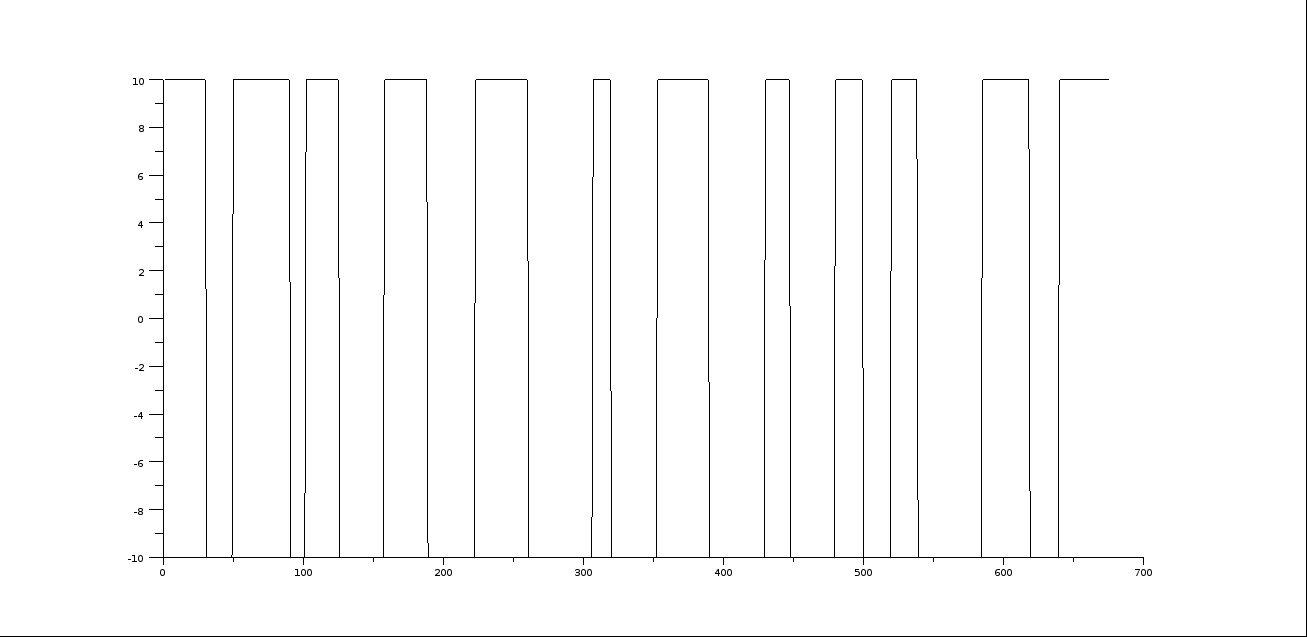
\includegraphics[width=0.7\linewidth]{prbs/prbs-illustration.png}
\caption{A Pseudo Random Binary Sequence}
\label{prbs-fig}
\end{figure}

\begin{figure}
\centering
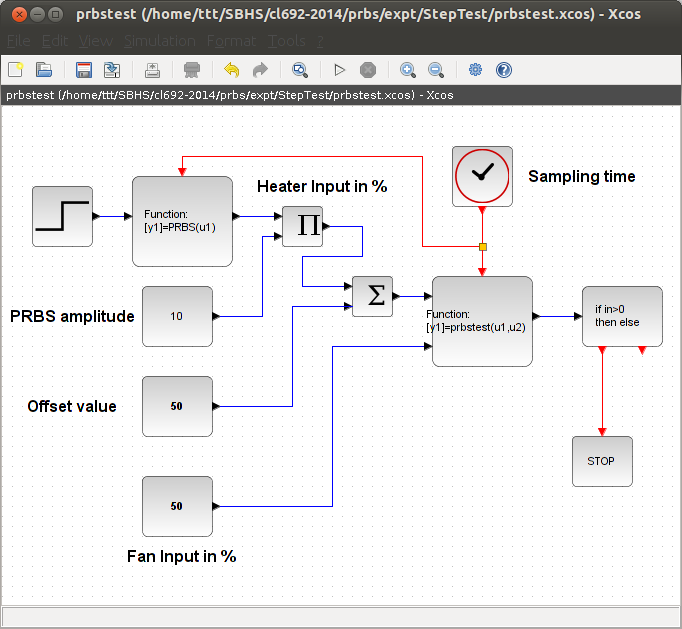
\includegraphics[width=0.7\linewidth]{prbs/prbs-xcos.png}
\caption{Xcos for PRBS testing experiment}
\label{prbs-xcos}
\end{figure}


System identification is carried out to identify the transfer function between the input signal to the system and output from the system. Firstly a transfer function with unknown parameters is assumed. The system is given a known input and its response is obtained and then the values of the unknown parameters is chosen such that the sum of squares of the errors is minimized. Here, the error is the difference between the actual output and the output predicted by the transfer function model assumed.



For the given SBHS system, we assume a second order transfer function:

\begin{equation}
G(z)=\frac{b_{1}+b_{2}z^{-1}}{1+a_{1}z^{-1}+a_{2}z^{-2}}z^{-d}
\end{equation}


The unknown parameters $a_1, a_2, b_1, b_2$ and d are to be obtained through the response of the system to the known inputs.  $a_1, a_2, b_1, b_2$ are real numbers and d is the plant delay which is an integer.  For these model parameters estimation, we used a pseudo random binary sequence (PRBS) input. Since the optimization over discrete variables (d in this case) is a very difficult routine for computers, we assume a value of d and then optimize over  $a_1, a_2, b_1, b_2$. The optimization problem, then, becomes:



\[
(\hat{b_1}, \hat{b_2}, \hat{a_1}, \hat{a_2})=\underset{b_1, b_2, a_1, a_2}{argmin}\sum_{i=0}^{N}(y(k)-\hat{y}(k))^{2}
\]

Here, $y(k)$ is the output obtained from the system, so it is known, $\hat{y(k)}$ is the estimated output using $y$ the model assumed, which can be written as a difference equation:

\begin{align}
\hat{y}(k) = -a_1\hat{y}(k - 1) - a_2\hat{y}(k - 2) + b_1 u(k - d) + b_2 u(k - 1 - d)
\end{align}

The optimization is performed using the optimization routine “optim” of Scilab.




\subsection{Implementing IMC controller on SBHS, virtually}
The step by step procedure for conducting an experiment virtually is explained in section \ref{vlabsexpt}. The required .sce file is {\tt imc\_virtual.sce}.  You will find this file in the {\tt imc\_controller} directory under {\tt virtual} folder. The necessary codes are listed in the section \ref{imccodes}


\section{Scilab Code}\label{imccodes}
\begin{code}
\ccaption{ser\_init.sce}{\ttfamily ser\_init.sce}
\lstinputlisting{Scilab/local/imc_controller/ser_init.sce}
\end{code}

\begin{code}
 \ccaption{imc.sci}{\ttfamily imc.sci}
\lstinputlisting{Scilab/local/imc_controller/imc.sci}
\end{code}


\begin{code}
 \ccaption{imc\_virtual.sce}{\ttfamily imc\_virtual.sce}
\lstinputlisting{Scilab/virtual/imc_controller/imc_virtual.sce}
\end{code}


\begin{code}
 \ccaption{imc\_virtual.sci}{\ttfamily imc\_virtual.sci}
\lstinputlisting{Scilab/virtual/imc_controller/imc_virtual.sci}
\end{code}


%\bibliography{imc} 
